\pdfminorversion=7
\begin{filecontents*}[overwrite]{\jobname.xmpdata}
    \Title{Szilágyi Gábor - Önéletrajz}
    \Author{Szilágyi Gábor}
    \Language{hu-HU}
    \Subject{Önéletrajz beadva ide: thyssenkrupp Components Technology Hungary kft.}
    \Keywords{önéletrajz, thyssenkrupp}	% \sep does not seem to work, only commas
\end{filecontents*}

\documentclass[a4paper,12pt,onesize,oneside,unicode,titlepage]{article}
% CV in LaTeX

%% PACKAGES %%

\usepackage[english]{babel} % multilingual support
\usepackage[utf8]{inputenc} % encoding
\usepackage[T1]{fontenc} % for PDF/A
\usepackage{tgpagella} % Set the default font
\usepackage{graphicx} % Set the default font
\usepackage{background}
\usepackage{tikz}
\usepackage[pdfa]{hyperref} % For Hyperlinks
\usepackage[a-3u,mathxmp]{pdfx} % for PDF/A
\usepackage{colorprofiles} % for PDF/A
\usepackage{enumitem}
\usepackage{geometry}
\usepackage{titlesec}
\titleformat*{\section}{\large\bfseries\vspace{2.7ex}\titlerule\vspace{-2.7ex}}
    %\sectionrule{0pt}{0pt}{-5pt}{1pt} % insert a thin rule
% spacing before and after a section
%\titlespacing*{\section}{0pt}{.2ex}{.2ex}
%\titleformat*{\section}{\large\bfseries}

\setlist[itemize]{itemsep=0.5ex, topsep=0pt} % enumitem setup
% set the page layout
\geometry{
    a4paper,
    left=15mm,
    right=15mm,
    bottom=0mm,
    top=10mm}

% empty the headers, footers, pagenumbers…
\pagestyle{empty}

\hypersetup{
    pdfstartview=,			% select PDF viewer default view explicitly, to avoid PDF/A violation
    colorlinks=true,           % false: boxed links; true: colored links
    linkcolor=black,           % color of internal links
    citecolor=black,           % color of links to bibliography
    filecolor=black,           % color of file links
    urlcolor=black,             % color of external links
    pdfnewwindow=true,         % links in new window
}

\makeatletter
\def\PAX@attrs@URI#1{/F 4 #1}
\makeatletter

%% MACROS %%

% size of the boxes used to align text
\newlength{\spacebox}
\settowidth{\spacebox}{123456789}

% vertical space separator between entries
\newcommand{\sepspace}{\vspace*{1em}}

% name
\newcommand{\name}[1]{
    \Huge % font size
    \fontfamily{phv}\selectfont % font family
    % print name centered and bold
    \begin{center} \textbf{#1} \end{center}\par
    % back to normal size and font
    \normalsize\normalfont}

% motto
\newcommand{\motto}[1]{
    \large % font size
    \fontfamily{phv}\selectfont % font family
    % print motto centered and slanted
    \begin{center} \textsl{#1}\end{center}\par
    % back to normal size and font
    \normalsize \normalfont}

% personal information
\newcommand{\info}[2]{
    % set specific indentation for personal information
    \noindent\hangindent=2em\hangafter=0
    % create a box to align two pieces of text
    \parbox{\spacebox}{%
        \textsl{#1}} % slanted entry name
    #2 \par} % entry value

% skill
\newcommand{\skill}[2]{
    % set specific indentation for personal information
    \noindent\hangindent=2em\hangafter=0
    % create a box to align two pieces of text
    \parbox{3\spacebox}{% three times larger box
        \textsc{#1}} % small caps entry name
    #2 \par} % entry value

% language level
\newcommand{\lan}[2]{
    \textbf{#1}\quad--\quad#2}    % entry value

% education entry
\newcommand{\education}[4]{
    % name of the studies
    \noindent  {\bfseries#1}
    % at the right the duration
    \hfill 
    \framebox{% duration inside a frame box
        \parbox{6em}{%
            \centering{\bfseries#2}}} \par
    % new paragraph with the school in italics
    \noindent {\itshape#3} \par
    % description with no hanging and in smaller text
    \vspace*{0.5em}
    \noindent\hangindent=2em\hangafter=0 \small #4
    %back to normal size
    \normalsize \par}

% work experience

\newcommand{\work}[4]{
    % name of the work
    \noindent  {\bfseries#1}
    % at the right the duration
    \hfill 
    \framebox{% duration inside a frame box
        \parbox{6em}{%
            \centering{\bfseries#2}}} \par
    % new paragraph with the school in italics
    \noindent {\itshape#3} \par
    % description with no hanging and in smaller text
    \vspace*{0.5em}
    \noindent\hangindent=2em\hangafter=0 \small #4
    %back to normal size
    \normalsize \par}

\newcommand{\MyGraphicLogo}{% For imported graphic logo
    \begin{tikzpicture}[remember picture,overlay,yshift=-3cm, xshift=-3.5cm]
    \node at (0,0) {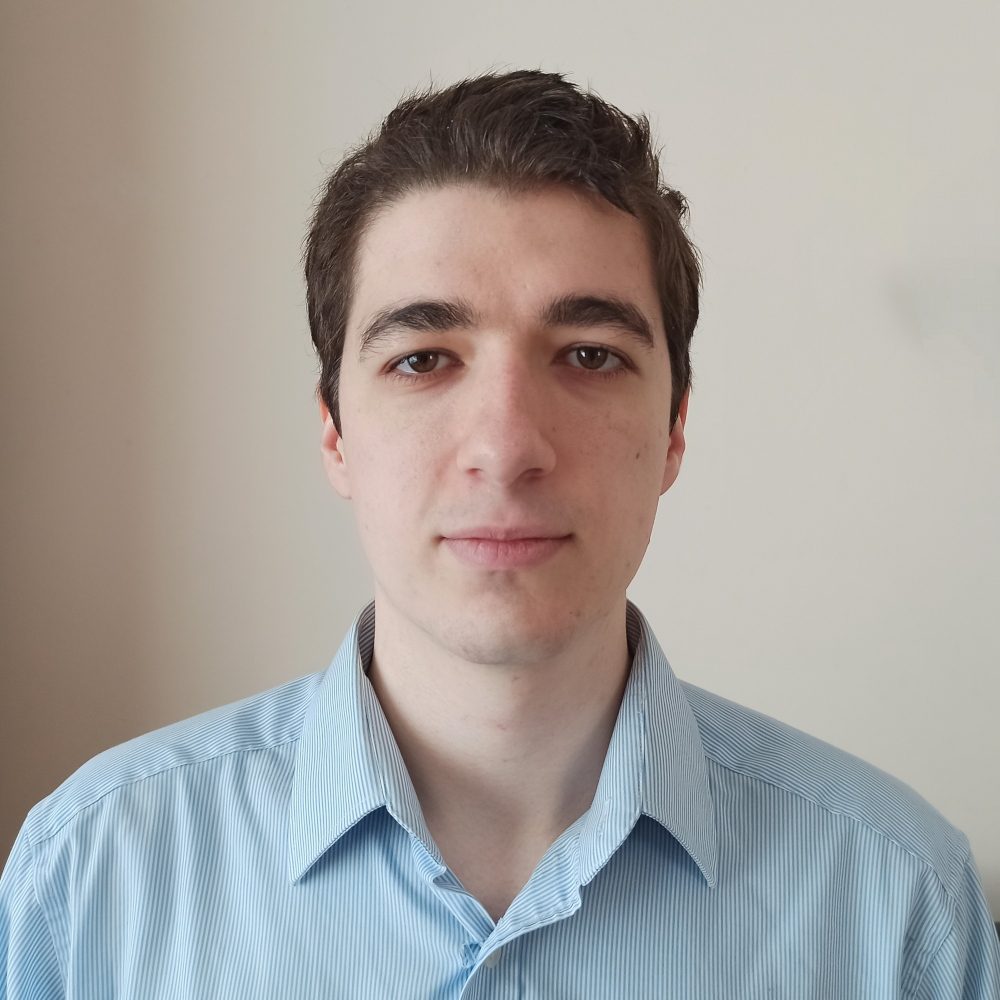
\includegraphics[width=4cm]{gabor_kicsi.jpg}};
    \end{tikzpicture}
}

\SetBgContents{\MyGraphicLogo}% Select included image

\SetBgPosition{current page.north east}% Select location
\SetBgOpacity{1.0}% Select opacity
\SetBgAngle{0.0}% Select roation of logo
\SetBgScale{1.0}% Select scale factor of logo

\begin{document}
% name and motto
\name{Gábor Szilágyi}
%\vspace*{-10pt}
%\motto{Work is my motivation}
% personal information
%\sepspace
\info{Email}{\href{mailto:gbr.szilagyi@gmail.com}{gbr.szilagyi@gmail.com}}
\info{Phone}{\href{tel:+36307568542}{+36 30 756 8542}}
\info{LinkedIn}{\href{https://www.linkedin.com/in/gabor-szilagyi-0b4b4720b/}{Gabor Szilagyi}}
\info{Address}{1032 Budapest, Kiscelli utca 16, 7/40}
\info{Birth}{1999.05.18.}
% education
\section*{Education}
    \education{Master's Degree in Electrical Engineering}{2022--2024}{Budapest University of Technology and Economics}{Department of Broadband Infocommunications and Electromagnetic Theory\\FPGA Based Systems (auxiliary specialization)\vspace{2ex}
    }
    \education{Bachelor's Degree in Electrical Engineering}{2018--2022}{Budapest University of Technology and Economics}{Department of Broadband Infocommunications and Electromagnetic Theory}
% work experience
\section*{Work Experience}
    \work{Hardware Intern}{2021--2022}{Silicon Laboratories Hungary kft.}{
        \begin{itemize} \setlength\itemsep{0.5ex}
            \item RF measurements at the on-site antenna chamber, measurement automation in Python
            \item Soldering tasks (mostly fine-tuning of matching/filter networks)
            \item PCB design in Altium, Schematic/BOM management
        \end{itemize}}
    \work{Hardware Intern}{2023--2024}{thyssenkrupp Components Technology Hungary kft.}{
        \begin{itemize} \setlength\itemsep{0.5ex}
            \item Worst case analysis of automotive electronics
            \item PCB design in Altium
            \item Temperature chamber measurements
        \end{itemize}}
% technical skills
\section*{Technical skills}
    \skill{Programming languages}{\textsc{C}, \textsc{C++}, \textsc{MATLAB}, \LaTeX, \textsc{Python}, \textsc{Rust}}
    \skill{Other}{\textsl{Git, Vim, Linux, Altium, LTspice, Amateur Radio lincense}}
% languages
\section*{Languages}
    \lan{Hungarian}{native}
    \hfill
    \lan{English}{C1}
    \hfill
    \lan{German}{A1}
% Social competencies
\section*{Social competencies}
    \begin{itemize} \setlength\itemsep{0.5ex}
        \item I consider myself very empathic
        \item Experience as the team leader of the HA5KFU amateur radio club in the Simonyi Károly Szakkollégium
        \item I can work efficiently both in teams and alone
    \end{itemize}
\end{document}